\documentclass{beamer}
\usetheme{Boadilla}
\usecolortheme{seahorse}
\usefonttheme{professionalfonts}
\usepackage{lmodern}
\setbeamerfont{normal text}{family=\sffamily}
\setbeamerfont{frametitle}{family=\sffamily,size=\large}
\setbeamerfont{footline}{family=\sffamily,size=\tiny}

\usepackage{graphicx,xcolor}
\usepackage{amsmath,amssymb,amsfonts,bm}
\usepackage{booktabs,array,tabularx,multirow}
\usepackage{tikz}
\usetikzlibrary{arrows.meta,positioning,shapes.geometric,fit,calc}
\usepackage{hyperref}

\setbeamertemplate{caption}[numbered]
\setbeamertemplate{blocks}[rounded][shadow=false]
\setbeamertemplate{navigation symbols}{}
\setbeamertemplate{footline}{%
  \leavevmode\hbox{%
    \begin{beamercolorbox}[wd=.333333\paperwidth,ht=2.6ex,dp=1ex,center]{author in head/foot}%
      \usebeamerfont{footline}\insertshortauthor
    \end{beamercolorbox}%
    \begin{beamercolorbox}[wd=.333333\paperwidth,ht=2.6ex,dp=1ex,center]{title in head/foot}%
      \usebeamerfont{footline}%
      \ifnum\insertframenumber=1 Overview\else
        \ifx\insertsubsectionhead\empty
          \insertsectionhead
        \else
          \insertsubsectionhead
        \fi
      \fi
    \end{beamercolorbox}%
    \begin{beamercolorbox}[wd=.333334\paperwidth,ht=2.6ex,dp=1ex,right]{date in head/foot}%
      \usebeamerfont{footline}\insertframenumber{} / \inserttotalframenumber\hspace*{1em}
    \end{beamercolorbox}%
  }%
}
\setbeamertemplate{title page}[default]
\graphicspath{{images/}{images/eda/}{images/modwt/}{images/results/}{images/paper/}{images/logo/}{images/illustrate/}}

\title[WaveCatBoost]{WaveCatBoost: Hybrid Air Quality Forecasting}
\subtitle{Applied Time Series Analysis --- Course Project\\[0.4em]\textbf{Group 8}}
\author[Group 8]{%
  \texorpdfstring{%
    \begin{tabular}{@{}c@{\hspace{2.2em}}c@{}}
      Kumar Utkarsh & P~Sai Deva Charan \\[-0.15em]
      {\footnotesize 240150016} & {\footnotesize 240150024} \\[0.85em]
      M~Charan Sree Teja & D~Lalit Santosh \\[-0.15em]
      {\footnotesize 240150018} & {\footnotesize 240150044}
    \end{tabular}%
  }{Group 8}%
}
\date{}

\begin{document}

\begin{frame}
  \titlepage
\end{frame}

\section{Problem and Approach}
\begin{frame}{Problem and Approach}
  \begin{block}{Why this is hard}
    \begin{itemize}
      \item Air-quality forecasting needs \textbf{near real-time} answers.
      \item That pushes us toward \textbf{lighter} models (trees, short lags).
      \item The series is \textbf{non-stationary}: spikes, regime shifts, and changing variance.
      \item Light models struggle on the \textbf{raw} mix of spikes, diurnal cycles, and slow drift.
    \end{itemize}
  \end{block}

  \begin{exampleblock}{Paper approach}
    \begin{enumerate}
      \item Split the series into scale-wise components (details + smooth) with Haar MODWT.
      \item Forecast each component with CatBoost.
      \item Reconstruct by summing bands; optionally add conformal intervals.
    \end{enumerate}
  \end{exampleblock}
\end{frame}


\section{Datasets and Preprocessing}
\begin{frame}{Datasets}
  \begin{columns}[T]
    \begin{column}{0.38\textwidth}
      {\footnotesize
      \textbf{Paper CSVs (Meghalaya, hourly)}
      \begin{itemize}\setlength\itemsep{0.15em}
        \item \textbf{CPCB}, \textbf{ID1} from Borah et al.
        \item $n \approx 8880$ / $9505$.
        \item NO$_2$, O$_3$, CO, SO$_2$, PM$_{2.5}$, PM$_{10}$.
      \end{itemize}
      \textbf{Extra CAAQMS (15-min $\to$ hourly)}
      \begin{itemize}\setlength\itemsep{0.15em}
        \item \textbf{Shillong:} Lumpyngngad.
      \end{itemize}
      }
    \end{column}
    \begin{column}{0.60\textwidth}
      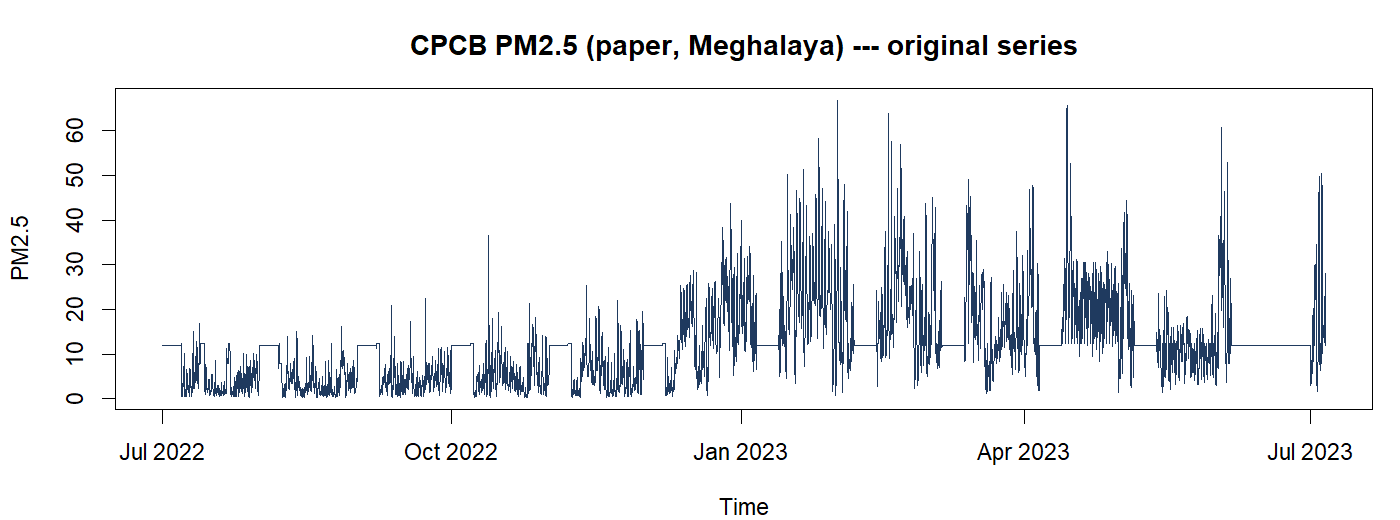
\includegraphics[width=\linewidth]{series_cpcb_pm25.png}\\[-0.2em]
      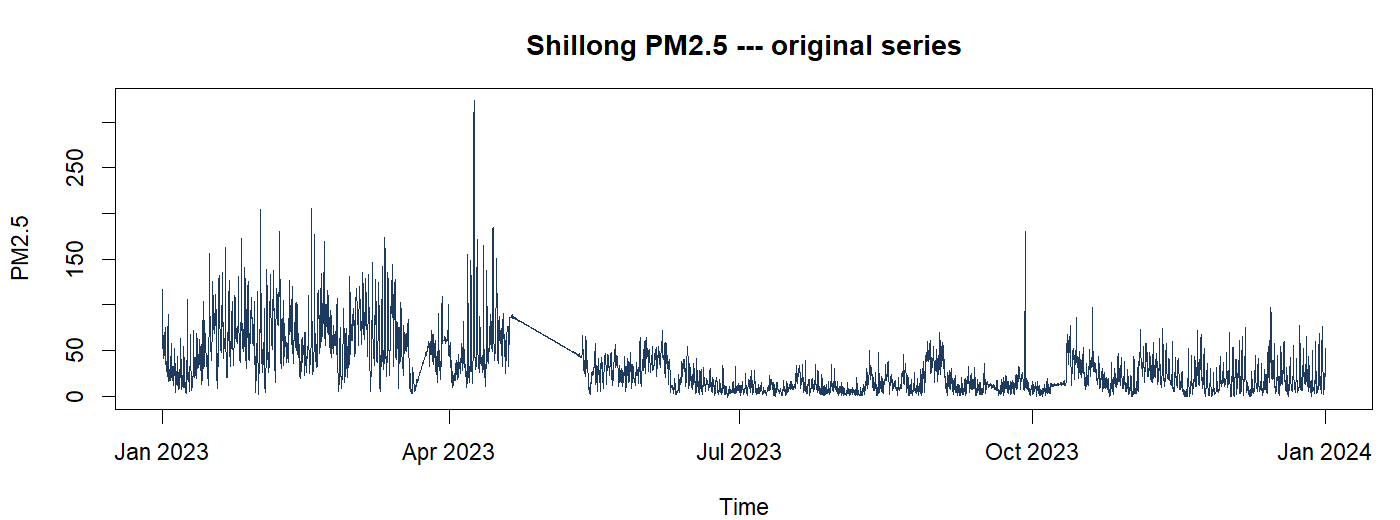
\includegraphics[width=\linewidth]{series_shillong_pm25.png}
    \end{column}
  \end{columns}
\end{frame}

\begin{frame}{Dataset diagnostics --- ACF / PACF}
  \begin{columns}[c]
    \begin{column}{0.52\textwidth}
      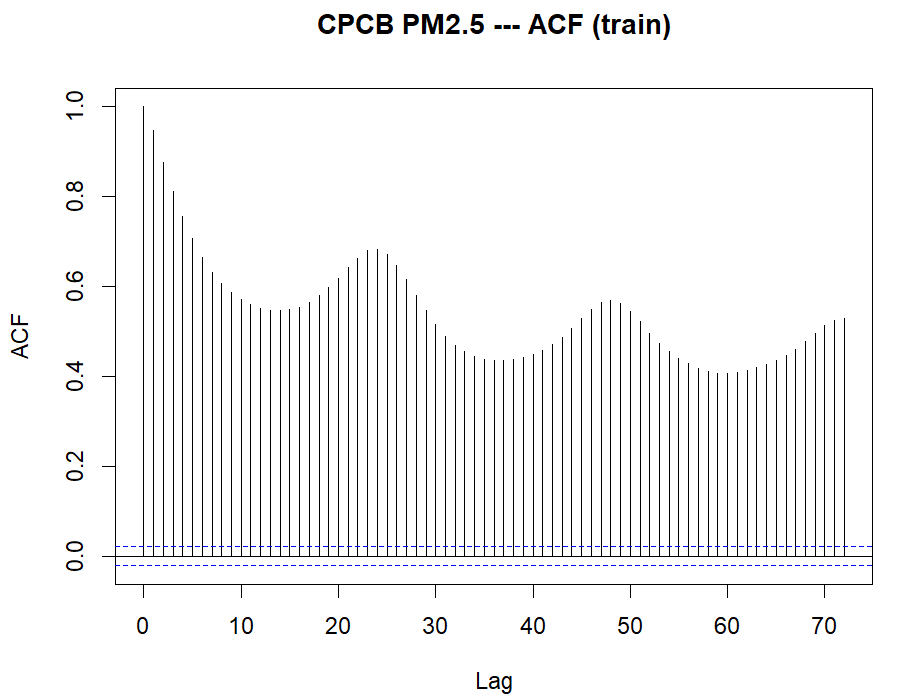
\includegraphics[width=\linewidth,height=0.38\textheight,keepaspectratio]{acf_cpcb_pm25.png}
    \end{column}
    \begin{column}{0.46\textwidth}
      {\footnotesize
      \textbf{ACF}\\[0.25em]
      Correlation of \(Y_t\) with \(Y_{t-k}\) for lags up to 72.\\[0.35em]
      Stays high and waves every \(\sim 24\) lags \(\Rightarrow\) strong daily seasonality plus long memory (yesterday's level still matters).
      }
    \end{column}
  \end{columns}
  \vspace{0.35em}
  \begin{columns}[c]
    \begin{column}{0.52\textwidth}
      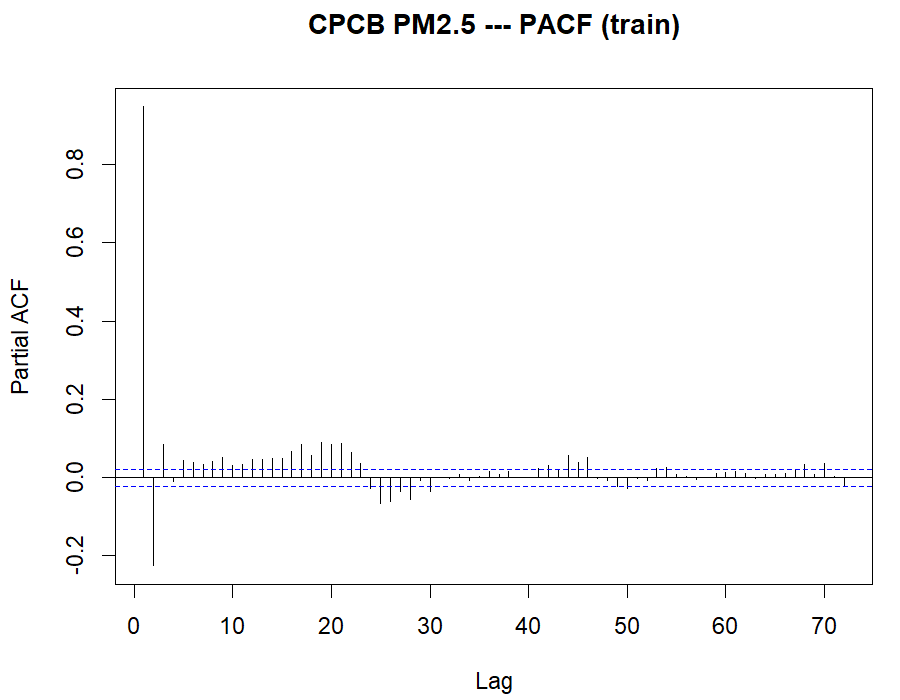
\includegraphics[width=\linewidth,height=0.38\textheight,keepaspectratio]{pacf_cpcb_pm25.png}
    \end{column}
    \begin{column}{0.46\textwidth}
      {\footnotesize
      \textbf{PACF}\\[0.25em]
      ``Extra'' correlation after earlier lags are accounted for.\\[0.35em]
      Huge spike at lag~1, then mostly small \(\Rightarrow\) strongest short-term link is the previous hour (AR-style / lag-1 features). Lag~24 shows more in the ACF than as a big PACF spike.
      }
    \end{column}
  \end{columns}
\end{frame}

\begin{frame}{Dataset diagnostics --- lag scatters}
  \begin{columns}[c]
    \begin{column}{0.52\textwidth}
      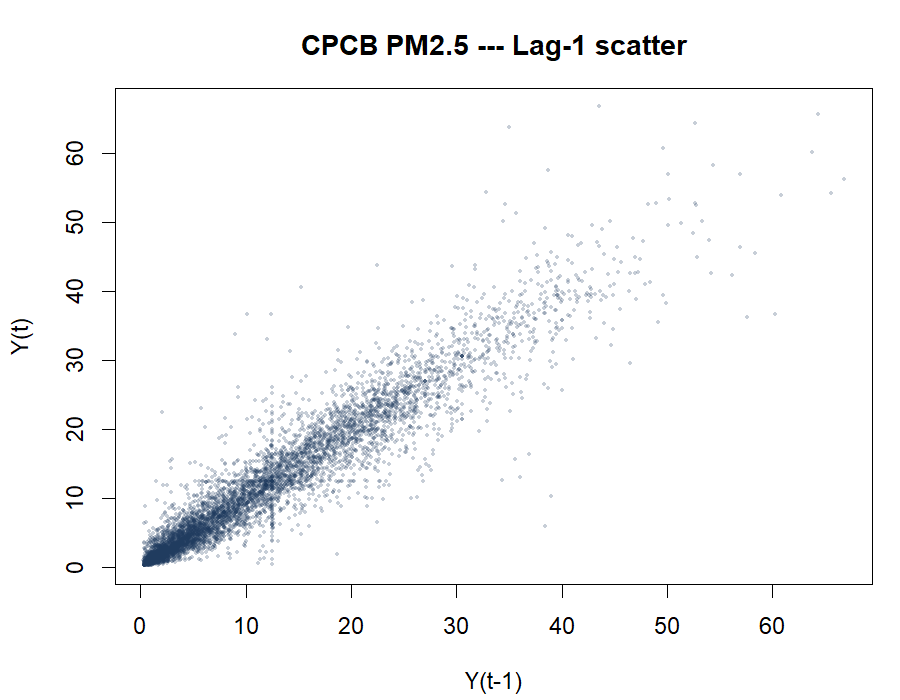
\includegraphics[width=\linewidth,height=0.38\textheight,keepaspectratio]{lag1_scatter_cpcb_pm25.png}
    \end{column}
    \begin{column}{0.46\textwidth}
      {\footnotesize
      \textbf{Lag-1 scatter}\\[0.25em]
      \(Y_t\) vs \(Y_{t-1}\): tight diagonal.\\[0.35em]
      Next hour is usually close to this hour \(\Rightarrow\) high persistence / smooth hour-to-hour changes.
      }
    \end{column}
  \end{columns}
  \vspace{0.35em}
  \begin{columns}[c]
    \begin{column}{0.52\textwidth}
      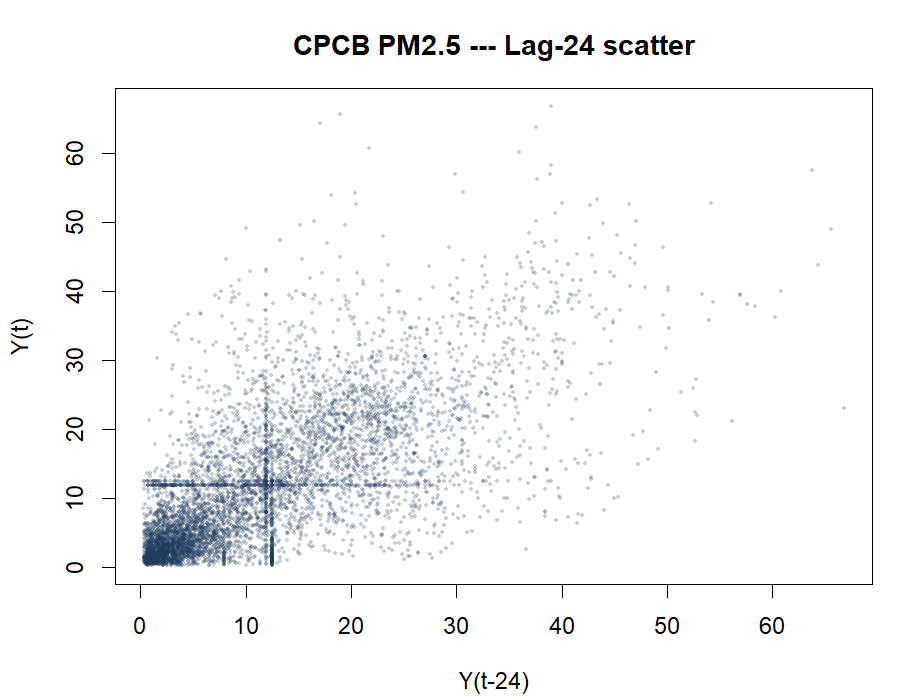
\includegraphics[width=\linewidth,height=0.38\textheight,keepaspectratio]{lag24_scatter_cpcb_pm25.png}
    \end{column}
    \begin{column}{0.46\textwidth}
      {\footnotesize
      \textbf{Lag-24 scatter}\\[0.25em]
      \(Y_t\) vs \(Y_{t-24}\): still positive (same hour yesterday helps), but much looser than lag~1.\\[0.35em]
      Daily cycle is real, but weaker than the immediate lag.
      }
    \end{column}
  \end{columns}
\end{frame}

\begin{frame}{Seasonal structure --- CPCB PM$_{2.5}$}
  \centering
  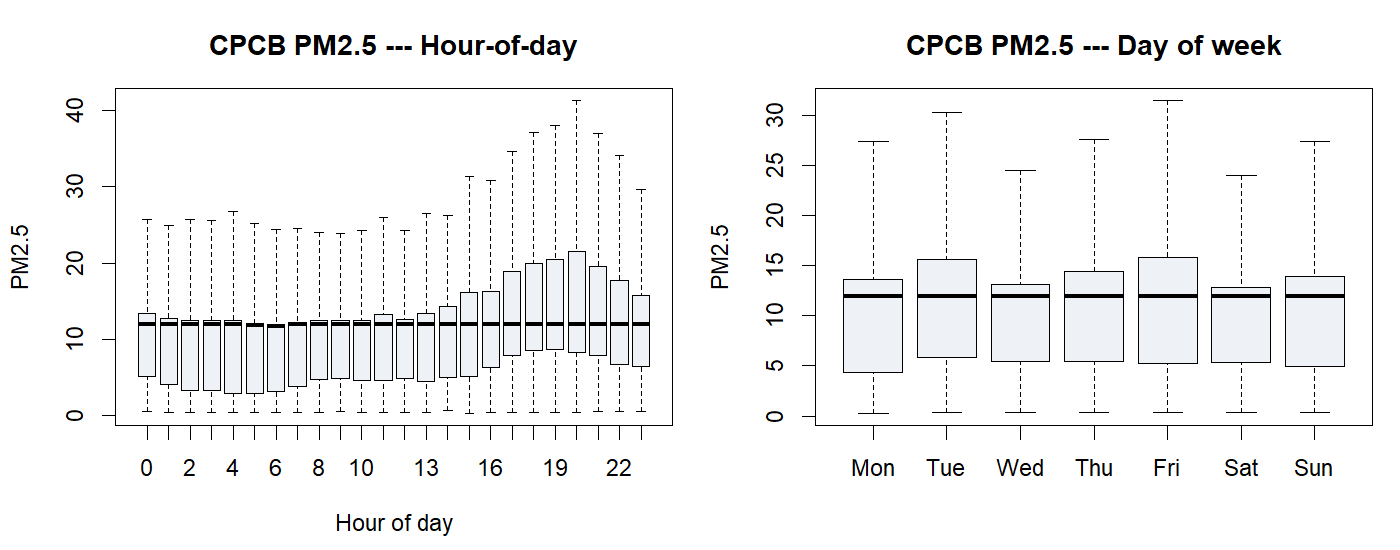
\includegraphics[width=0.95\linewidth,height=0.62\textheight,keepaspectratio]{boxes_cpcb_pm25.png}
  \vspace{0.15em}
  \begin{itemize}\setlength\itemsep{0.2em}
    \item Clear diurnal pattern; milder weekday effect.
    \item $S$ = \textbf{seasonality period} (hours in one cycle). Here $S{=}24$ = one day.
    \item Used for seasonal naive, SARIMA seasonal lag, and the MASE denominator.
    \item Also motivates lag features up to 24~h.
  \end{itemize}
\end{frame}

\begin{frame}{What we did before modelling}
  \begin{itemize}
    \item \textbf{Hourly grid:} end-labelled hourly means (15-min CAAQMS $\to$ hour $t$).
    \item \textbf{Quality screen:} physical bounds, stuck sensors, spike flags.
    \item \textbf{Causal fill:} impute only with information available up to the cut time.
    \item \textbf{Chronological split:} train $\to$ val (14\,d tuning) $\to$ test (last $h$ hours);\\
          $h\in\{24,168,336,744\}$. No random split.
    \item \textbf{Scale:} min--max to $[0,1]$ fit on \textbf{train only}.
    \item Paper Meghalaya CSVs are already hourly $\Rightarrow$ skip re-aggregation / fill.\\
          Extra Shillong data get the full clean path into an isolated store.
  \end{itemize}
\end{frame}


\section{MODWT Decomposition}
\begin{frame}{Why decompose? Why not Fourier?}
  \begin{block}{Why split the series}
    \begin{itemize}
      \item Raw $Y_t$ mixes noise, diurnal swings, and slow level shifts.
      \item One light model on the mix misses scale-specific structure.
      \item Decompose $\to$ forecast each band $\to$ add back $=$ richer dynamics without a heavy global model.
    \end{itemize}
  \end{block}
  \begin{alertblock}{Why not Fourier}
    \begin{itemize}
      \item Fourier uses \textbf{global} sinusoids over the whole record.
      \item Air quality is \textbf{non-stationary} --- spikes and regime changes are local in time.
      \item Wavelets give a joint \textbf{time--scale} view; MODWT keeps every band length $N$ (no downsampling).
      \item MODWT MRA is additive for Haar, D4, LA8, \ldots:
            $Y_t=\sum_k D_{k,t}+S_{K,t}$ (paper uses Haar).
    \end{itemize}
  \end{alertblock}
\end{frame}

\begin{frame}{MODWT: additive components}
  \begin{columns}[T]
    \begin{column}{0.40\textwidth}
      \[
        Y_t = \sum_{k=1}^{K} D_{k,t} + S_{K,t}
      \]
      {\footnotesize
      \begin{itemize}
        \item $D_{k,t}$: detail at scale $\sim 2^{k}$~h.
        \item $S_{K,t}$: smooth after $K$ levels.
        \item Paper: $K\approx\ln N$; we use $K{=}4$--$5$ ($\sim 16$--$32$~h smooth).
        \item $D_1$: high-frequency component;\\
              $D_k$: lower-frequency component;\\
              $S_K$: smooth trend / level.
      \end{itemize}
      }
    \end{column}
    \begin{column}{0.58\textwidth}
      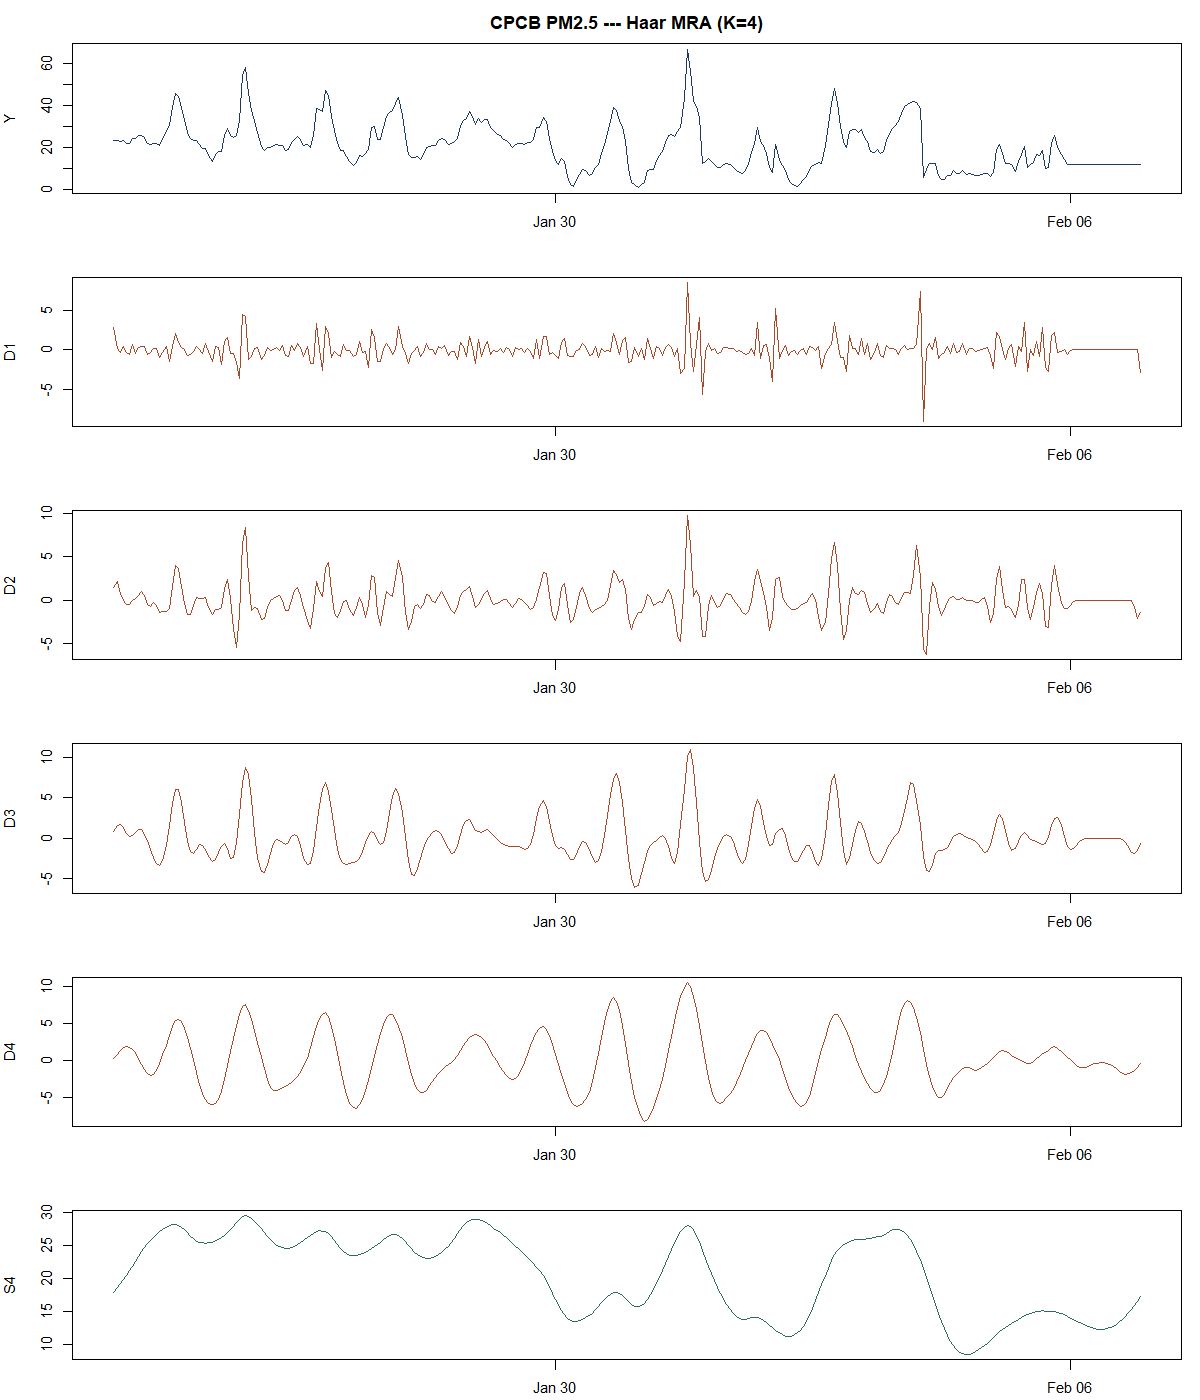
\includegraphics[width=\linewidth,height=0.78\textheight,keepaspectratio]{mra_d1d4_s4_cpcb_pm25.png}
    \end{column}
  \end{columns}
\end{frame}

% Mathematical intuition --- boxed filters like reference slide; compact tree
\begin{frame}{MODWT: mathematical intuition}
  \begin{columns}[T]
    \begin{column}{0.50\textwidth}
      {\scriptsize
      \noindent
      \fcolorbox{gray!55}{gray!12}{\parbox{0.96\linewidth}{%
        \textbf{Wavelet filter:} $p_m\to D$ (details)\\
        $\sum_m p_m=0$ \ (measures change)}}\\[0.3em]
      \fcolorbox{gray!55}{gray!12}{\parbox{0.96\linewidth}{%
        \textbf{Scaling filter:} $q_m\to S$ (smooth)\\
        $\sum_m q_m=1$ \ (measures average)}}\\[0.4em]
      \textbf{Filter condition} (nonzero $n$):\\
      $\sum_m p_m p_{m+2n}=\sum_m q_m q_{m+2n}=0$\\[0.35em]
      \textbf{Recursion at level $j$}\ ($S_{0,t}=Y_t$)\\[0.15em]
      $D_{j,t}=\sum_{m}p_m\,S_{j-1,(t-2^{j-1}m)\bmod N}$\\[0.1em]
      $S_{j,t}=\sum_{m}q_m\,S_{j-1,(t-2^{j-1}m)\bmod N}$\\[0.25em]
      Haar: $q=(\tfrac12,\tfrac12)$,\ $p=(\tfrac12,-\tfrac12)$.\\
      Tap spacing doubles each level.
      }
    \end{column}
    \begin{column}{0.48\textwidth}
      \centering
      \resizebox{0.88\linewidth}{!}{%
      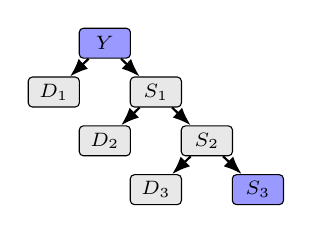
\begin{tikzpicture}[
        font=\scriptsize,
        x=0.72cm, y=0.62cm,
        box/.style={draw, rounded corners=1.5pt, align=center,
                    inner sep=1.2pt, minimum width=0.65cm, minimum height=0.38cm},
        ybox/.style={box, fill=blue!40},
        dbox/.style={box, fill=gray!18},
        sbox/.style={box, fill=gray!18},
        arr/.style={-{Latex}, thick}
      ]
        \node[ybox] (y)  at (0.9, 0) {$Y$};
        \node[dbox] (d1) at (0.0,-1.0) {$D_1$};
        \node[sbox] (s1) at (1.8,-1.0) {$S_1$};
        \node[dbox] (d2) at (0.9,-2.0) {$D_2$};
        \node[sbox] (s2) at (2.7,-2.0) {$S_2$};
        \node[dbox] (d3) at (1.8,-3.0) {$D_3$};
        \node[ybox] (s3) at (3.6,-3.0) {$S_3$};
        \draw[arr] (y)  -- (d1);
        \draw[arr] (y)  -- (s1);
        \draw[arr] (s1) -- (d2);
        \draw[arr] (s1) -- (s2);
        \draw[arr] (s2) -- (d3);
        \draw[arr] (s2) -- (s3);
      \end{tikzpicture}%
      }

      \vspace{0.2em}
      {\scriptsize
      Only the smooth is split again.\\
      $Y=D_1+D_2+D_3+S_3$\\[0.25em]
      \textbf{Inverse (IMODWT):} same filters, reversed\\
      \resizebox{\linewidth}{!}{$
        S_{j-1,t}=\sum_m p_m D_{j,t+2^{j-1}m}
        +\sum_m q_m S_{j,t+2^{j-1}m}
      $}
      }
    \end{column}
  \end{columns}
\end{frame}

\begin{frame}{Filter coefficients}
  \centering
  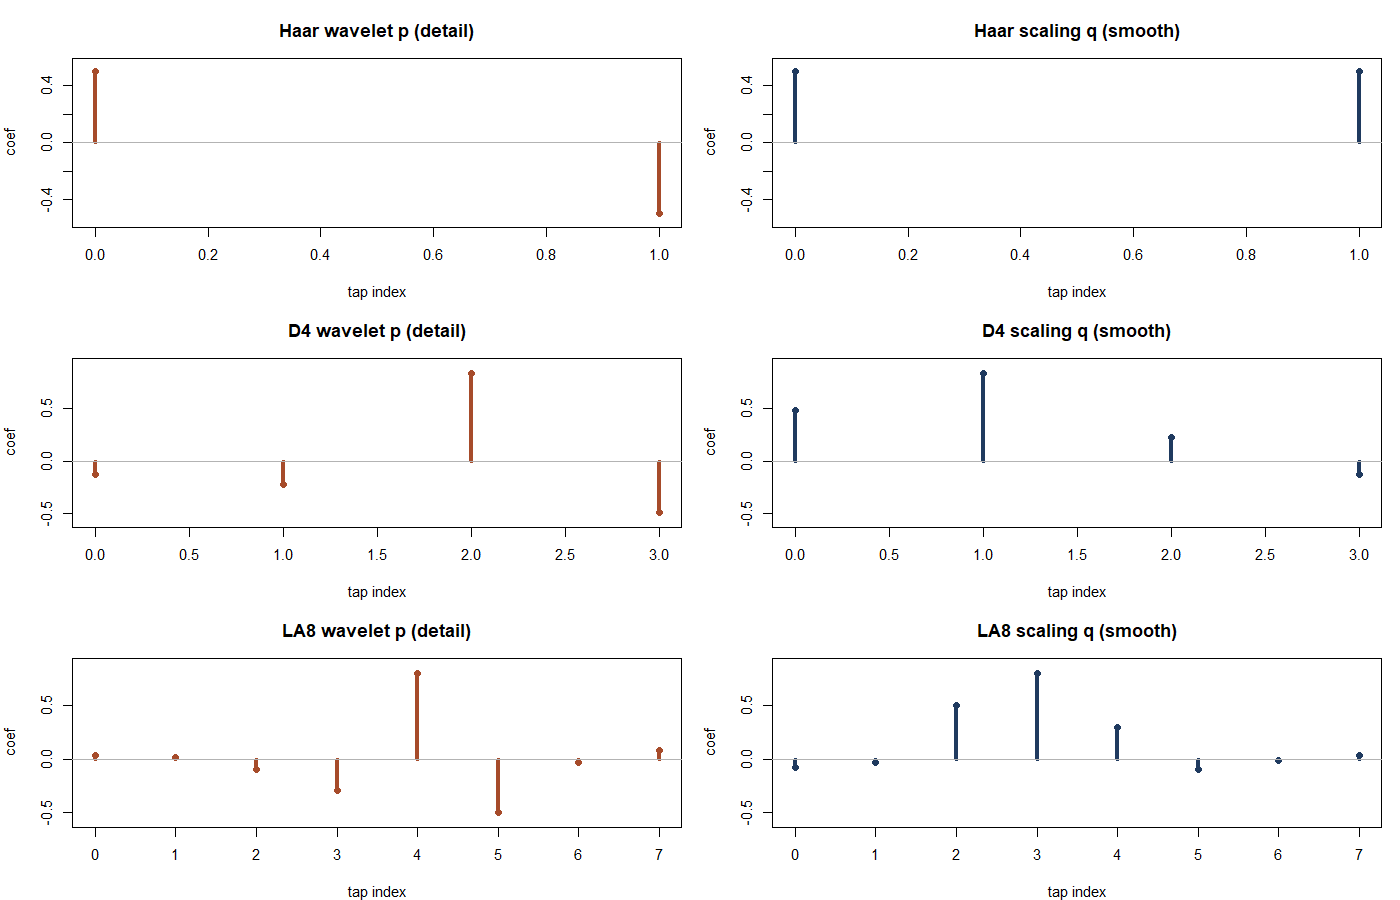
\includegraphics[width=0.95\linewidth,height=0.78\textheight,keepaspectratio]{filter_taps.png}
\end{frame}


\section{WaveCatBoost and Conformal Prediction}
\subsection{Model selection}
\begin{frame}{Which model to use?}
  \centering
  \resizebox{\linewidth}{!}{%
  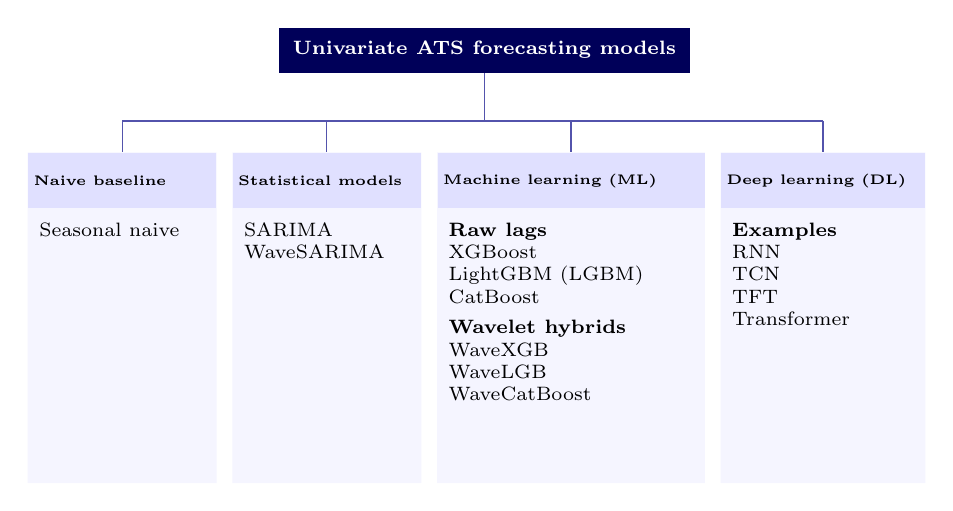
\begin{tikzpicture}[
    heading/.style={fill=blue!35!black,text=white,font=\scriptsize\bfseries,
                    inner sep=5pt},
    column title/.style={fill=blue!12,font=\tiny\bfseries,anchor=north west,
                         minimum height=0.7cm,align=left,inner xsep=2pt},
    body/.style={anchor=north west,font=\scriptsize,align=left,inner sep=4pt}
  ]
    \node[heading] (models) at (5.8,1.3) {Univariate ATS forecasting models};
    \draw[blue!35!gray] (models.south) -- (5.8,0.4)
      (1.2,0.4) -- (10.1,0.4)
      (1.2,0.4) -- (1.2,0)
      (3.8,0.4) -- (3.8,0)
      (6.9,0.4) -- (6.9,0)
      (10.1,0.4) -- (10.1,0);
    \fill[blue!4] (0,0) rectangle (2.4,-4.2)
                  (2.6,0) rectangle (5.0,-4.2)
                  (5.2,0) rectangle (8.6,-4.2)
                  (8.8,0) rectangle (11.4,-4.2);
    \node[column title,text width=2.25cm] at (0,0) {Naive baseline};
    \node[column title,text width=2.25cm] at (2.6,0) {Statistical models};
    \node[column title,text width=3.25cm] at (5.2,0) {Machine learning (ML)};
    \node[column title,text width=2.45cm] at (8.8,0) {Deep learning (DL)};
    \node[body] at (0,-0.75) {Seasonal naive};
    \node[body] at (2.6,-0.75) {SARIMA\\WaveSARIMA};
    \node[body] at (5.2,-0.75) {\textbf{Raw lags}\\XGBoost\\LightGBM (LGBM)\\CatBoost\\[0.4em]
      \textbf{Wavelet hybrids}\\WaveXGB\\WaveLGB\\WaveCatBoost};
    \node[body] at (8.8,-0.75) {\textbf{Examples}\\RNN\\TCN\\TFT\\Transformer};
  \end{tikzpicture}
  }
\end{frame}
% WaveCatBoost methodology + conformal prediction

\subsection{Error metrics}
\begin{frame}{Error metrics}
  \centering
  Mean absolute scaled error (MASE)\par\medskip
  $N$ is the training length, $h$ is the forecast horizon, and $S=24$ hours.
  \[
    \mathrm{MASE} = \frac{N-S}{h}\,
    \frac{\sum_{t=N+1}^{N+h}|\hat Y_t-Y_t|}
         {\sum_{t=S+1}^{N}|Y_t-Y_{t-S}|}.
  \]
  The denominator measures seasonal-naive error on the training data.
\end{frame}

\subsection{Model comparison}
\begin{frame}{Model comparison}
  \centering
  PM$_{2.5}$, 1-day horizon. Lower MASE is better.\par\medskip
  \definecolor{comparisonCPCB}{HTML}{474781}
  \definecolor{comparisonIDOne}{HTML}{8D9FCA}
  \resizebox{0.94\linewidth}{!}{%
  \begin{tikzpicture}[x=1cm,y=1cm,font=\scriptsize]
    \foreach \tick in {0,0.5,1,1.5,2} {
      \draw[gray!25,line width=0.3pt] (0,{1.3*\tick}) -- (10,{1.3*\tick});
      \node[left] at (0,{1.3*\tick}) {\tick};
    }
    \node[rotate=90] at (-0.7,1.3) {MASE};
    \foreach \x/\a/\b in {1/2.02/0.71,3/1.34/0.49,5/0.74/0.84,7/0.82/0.67,9/0.71/0.42} {
      \fill[comparisonCPCB] ({\x-0.38},0) rectangle ({\x-0.02},{1.3*\a});
      \fill[comparisonIDOne] ({\x+0.02},0) rectangle ({\x+0.38},{1.3*\b});
      \node[above,font=\tiny] at ({\x-0.2},{1.3*\a}) {\pgfmathprintnumber[fixed,precision=2]{\a}};
      \node[above,font=\tiny] at ({\x+0.2},{1.3*\b}) {\pgfmathprintnumber[fixed,precision=2]{\b}};
    }
    \node[below,align=center] at (1,-0.04) {Seasonal naive};
    \node[below] at (3,-0.04) {SARIMA};
    \node[below] at (5,-0.04) {LightGBM};
    \node[below] at (7,-0.04) {CatBoost};
    \node[below] at (9,-0.04) {WaveCatBoost};
    \fill[comparisonCPCB] (6.6,3.0) rectangle (6.9,3.15);
    \node[right] at (6.95,3.075) {CPCB};
    \fill[comparisonIDOne] (8.0,3.0) rectangle (8.3,3.15);
    \node[right] at (8.35,3.075) {ID1};
  \end{tikzpicture}%
  }
  \par\smallskip
  {\scriptsize
  \begin{tabular}{lrrrrr}
    \toprule
    Sensor & Seasonal naive & SARIMA & LightGBM & CatBoost & WaveCatBoost \\
    \midrule
    CPCB & 2.02 & 1.34 & 0.74 & 0.82 & \textbf{0.71} \\
    ID1 & 0.71 & 0.49 & 0.84 & 0.67 & \textbf{0.42} \\
    \bottomrule
  \end{tabular}
  }
\end{frame}

\subsection{CatBoost}
\begin{frame}{CatBoost: From Trees to Ordered Boosting}
  \small
  \textbf{1. Decision tree}
  \[
    f(x)=w_j \quad \text{if }x\in R_j
  \]
  Each leaf predicts a value.\par\smallskip
  \textbf{2. Gradient boosting}
  \[
    F_0(x)=c,\qquad
    r_i=y_i-F_{m-1}(x_i),\qquad h_m(x_i)\approx r_i
  \]
  \[
    F_m(x)=F_{m-1}(x)+\eta h_m(x),
    \qquad \eta\text{ is the learning rate.}
  \]
  \[
    h_m(x_i)\approx
    -\left.\frac{\partial L(y_i,F)}{\partial F}\right|_{F=F_{m-1}(x_i)}
  \]
  \textbf{3. Ordered boosting and symmetric trees}\par
  Ordered gradients use a model fitted on preceding observations.
  This reduces prediction shift.\par
  Same split at each depth. $2^d$ leaves, so $d=6\Rightarrow64$ leaves.
\end{frame}

\subsection{Hyperparameters}
\begin{frame}{Our Hyperparameters vs Original Paper}
  \small
  The paper followed a predefined protocol. We used a limited grid search
  to select the lag window, tree depth and learning rate.
  \medskip
  \centering
  {\scriptsize
  \begin{tabular}{lll}
    \toprule
    Parameter & Original paper & Our implementation \\
    \midrule
    Lag window ($p$) & 24 & $24,48 \rightarrow 24$ \\
    Wavelet depth ($K$) & $\lfloor\ln N\rfloor$, capped at 9 & 5 \\
    Tree depth & Default 6 & $4,6 \rightarrow 6$ \\
    Learning rate ($\eta$) & Automatic selection & $0.05,0.10 \rightarrow 0.05$ \\
    \bottomrule
  \end{tabular}
  }
  \[
    2\;(p)\times2\;(\mathrm{depth})\times2\;(\eta)
    =\boxed{8\text{ combinations}}
  \]
  \[
    \boxed{p=24,\quad \mathrm{depth}=6,\quad \eta=0.05}
  \]
  \begin{flushleft}
  \scriptsize
  Lag window: one daily cycle (24 h) versus two (48 h).\\
  Tree depth: 4 versus 6. Learning rate: 0.05 versus 0.10.\\
  Wavelet depth: $K=5$, using the energy-based choice and practical limits.
  The CPCB theoretical depth is $K=9$.\par\smallskip
  LightGBM selected the settings reused across the tree-based experiments.
  CatBoost was not independently tuned. The paper's core approach was retained.
  \end{flushleft}
\end{frame}

% ---- Conformal / uncertainty ----
\subsection{Conformal prediction}
\begin{frame}{Why conformal prediction?}
  \begin{columns}[c]
    \begin{column}{0.48\textwidth}
      \centering
      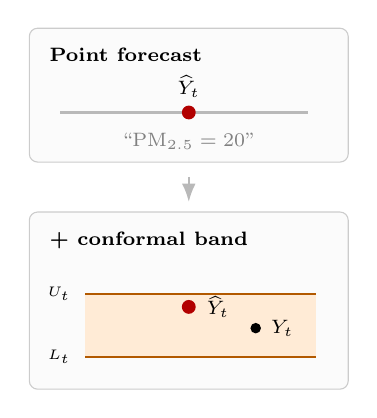
\begin{tikzpicture}[
        font=\scriptsize,
        >=Latex,
        panel/.style={draw=gray!40, rounded corners=3pt, inner sep=6pt,
                      fill=gray!3, minimum width=4.05cm}
      ]
        % ---- Panel 1: point forecast ----
        \node[panel, minimum height=1.7cm] (p1) {};
        \node[anchor=north west, font=\scriptsize\bfseries]
              at ([xshift=4pt,yshift=-4pt]p1.north west) {Point forecast};
        \draw[thick, gray!55] ([yshift=-0.22cm]p1.west) ++(0.4,0) -- ++(3.15,0);
        \coordinate (pf) at ([yshift=-0.22cm]p1.center);
        \fill[red!70!black] (pf) circle (2.5pt);
        \node[above=2pt] at (pf) {$\widehat Y_t$};
        \node[below=4pt, gray] at (pf) {``PM$_{2.5}=20$''};

        % ---- Arrow between panels ----
        \draw[-{Latex}, thick, gray!55] ([yshift=-0.18cm]p1.south) -- ++(0,-0.32);

        % ---- Panel 2: conformal band ----
        \node[panel, minimum height=2.25cm, below=0.62cm of p1] (p2) {};
        \node[anchor=north west, font=\scriptsize\bfseries]
              at ([xshift=4pt,yshift=-4pt]p2.north west) {+ conformal band};
        \fill[orange!16] ([xshift=0.72cm,yshift=-1.05cm]p2.north west)
              rectangle ([xshift=-0.42cm,yshift=0.42cm]p2.south east);
        \draw[thick, orange!70!black]
              ([xshift=0.72cm,yshift=-1.05cm]p2.north west)
              -- ([xshift=-0.42cm,yshift=-1.05cm]p2.north east);
        \draw[thick, orange!70!black]
              ([xshift=0.72cm,yshift=0.42cm]p2.south west)
              -- ([xshift=-0.42cm,yshift=0.42cm]p2.south east);
        \node[left=2pt, font=\tiny] at ([xshift=0.72cm,yshift=-1.05cm]p2.north west) {$U_t$};
        \node[left=2pt, font=\tiny] at ([xshift=0.72cm,yshift=0.42cm]p2.south west) {$L_t$};
        \coordinate (yh) at ([yshift=-0.08cm]p2.center);
        \coordinate (yt) at ([xshift=0.85cm,yshift=-0.35cm]p2.center);
        \fill[red!70!black] (yh) circle (2.5pt);
        \node[right=3pt] at (yh) {$\widehat Y_t$};
        \fill[black] (yt) circle (1.9pt);
        \node[right=2pt] at (yt) {$Y_t$};
      \end{tikzpicture}
    \end{column}
    \begin{column}{0.50\textwidth}
      {\footnotesize
      \begin{itemize}\setlength\itemsep{0.85em}
        \item \textbf{Need:} alerts need a safe range, not one risky guess.
        \item \textbf{Recipe:} use recent $|Y-\widehat Y|$ to set width ---
              large recent errors $\Rightarrow$ wider band.
        \item \textbf{No normal assumption:} AQ errors are spiky / quiet;
              conformal is distribution-free.
        \item \textbf{``95\%'':} about 95 of 100 hours, $Y_t\in[L_t,U_t]$
              (coverage).
      \end{itemize}
      }
    \end{column}
  \end{columns}
  \vspace{0.55em}
  {\footnotesize
  \centering
  From $\widehat Y_t$ alone to a band $[L_t,U_t]$ with target coverage $1-\alpha=95\%$.\par
  }
\end{frame}

\begin{frame}{Conformal formula}
  {\footnotesize
  \centering
  \renewcommand{\arraystretch}{1.35}
  \begin{tabular}{@{}r@{\hspace{0.7em}}c@{}}
    \textbf{Score}
      & $CS_t=\dfrac{|Y_t-\widehat Y_t|}{\widehat U_t}$ \\
    \textbf{Quantile}
      & $CQ_t=Q_{1-\alpha}\!\big(CS_{t-\kappa+1:t}\big)$ \\
    \textbf{Interval}
      & $PI_t=\widehat Y_t\pm CQ_t\,\widehat U_t$ \\
  \end{tabular}
  }
  \vspace{0.35em}
  {\scriptsize
  \centering
  Band edges:
  $L_t=\widehat Y_t-CQ_t\widehat U_t$,\
  $U_t=\widehat Y_t+CQ_t\widehat U_t$
  (clip $L_t\ge 0$).
  \par
  }
  \vspace{0.4em}
  \begin{columns}[T]
    \begin{column}{0.48\textwidth}
      {\footnotesize
      \begin{itemize}\setlength\itemsep{0.35em}
        \item $Y_t$, $\widehat Y_t$: truth / WaveCatBoost.
        \item $\widehat U_t$: local error scale (next slide).
        \item $CS_t$: scaled $|$error$|$ (nonconformity).
        \item $\alpha{=}0.05$ $\Rightarrow$ 95\% target.
        \item $\kappa\in\{24,168,336\}$~h (cal.\ window).
      \end{itemize}
      }
    \end{column}
    \begin{column}{0.50\textwidth}
      \begin{exampleblock}{How to use it}
        {\scriptsize
        \begin{enumerate}\setlength\itemsep{0.2em}
          \item Fit on train; residuals on a cal.\ window.
          \item Build $CS_t$; pick $\kappa$ for $\approx 95\%$ cal.\ coverage.
          \item Test: band $\widehat Y_t\pm CQ_t\widehat U_t$.
          \item Coverage $=$ share of $Y_t\in[L_t,U_t]$.
        \end{enumerate}
        }
      \end{exampleblock}
    \end{column}
  \end{columns}
\end{frame}

\begin{frame}{How $\widehat U_t$ and $CQ_t$ are computed}
  \begin{columns}[T]
    \begin{column}{0.48\textwidth}
      \begin{block}{$\widehat U_t$ --- local error scale}
        {\footnotesize
        Residual $e_t=Y_t-\widehat Y_t$.\\[0.35em]
        Default: \textbf{24-h rolling MAE}
        \[
          \widehat U_t=
          \operatorname{mean}\big(|e_{t-23}|,\ldots,|e_t|\big).
        \]
        Large recent mistakes $\Rightarrow$ large $\widehat U_t$
        $\Rightarrow$ wider band via $CQ_t\widehat U_t$.\\[0.35em]
        Multi-step test (no new $Y$ yet): freeze one robust
        $u^\star$ from calibration and reuse it.
        }
      \end{block}
    \end{column}
    \begin{column}{0.50\textwidth}
      \begin{block}{$CQ_t=Q_{1-\alpha}(CS_{t-\kappa+1:t})$}
        {\footnotesize
        \begin{enumerate}\setlength\itemsep{0.3em}
          \item Take the last $\kappa$ scores
                $CS_{t-\kappa+1},\ldots,CS_t$.
          \item Sort them.
          \item Take the $(1-\alpha)$-quantile
                ($\alpha{=}0.05$ $\Rightarrow$ $\approx$ 95th percentile).
        \end{enumerate}
        \vspace{0.25em}
        $CQ_t$ is the cutoff for a ``normal'' scaled error.\\
        Scores with $CS\le CQ_t$ fall inside
        $\widehat Y_t\pm CQ_t\widehat U_t$.
        }
      \end{block}
    \end{column}
  \end{columns}
\end{frame}

\begin{frame}{Do the intervals work? (7-day test)}
  {\footnotesize
  \textbf{Purpose:} letter-style 7-day PM$_{2.5}$ band --- does truth sit inside the
  95\% window around WaveCatBoost?
  }
  \vspace{0.3em}
  \centering
  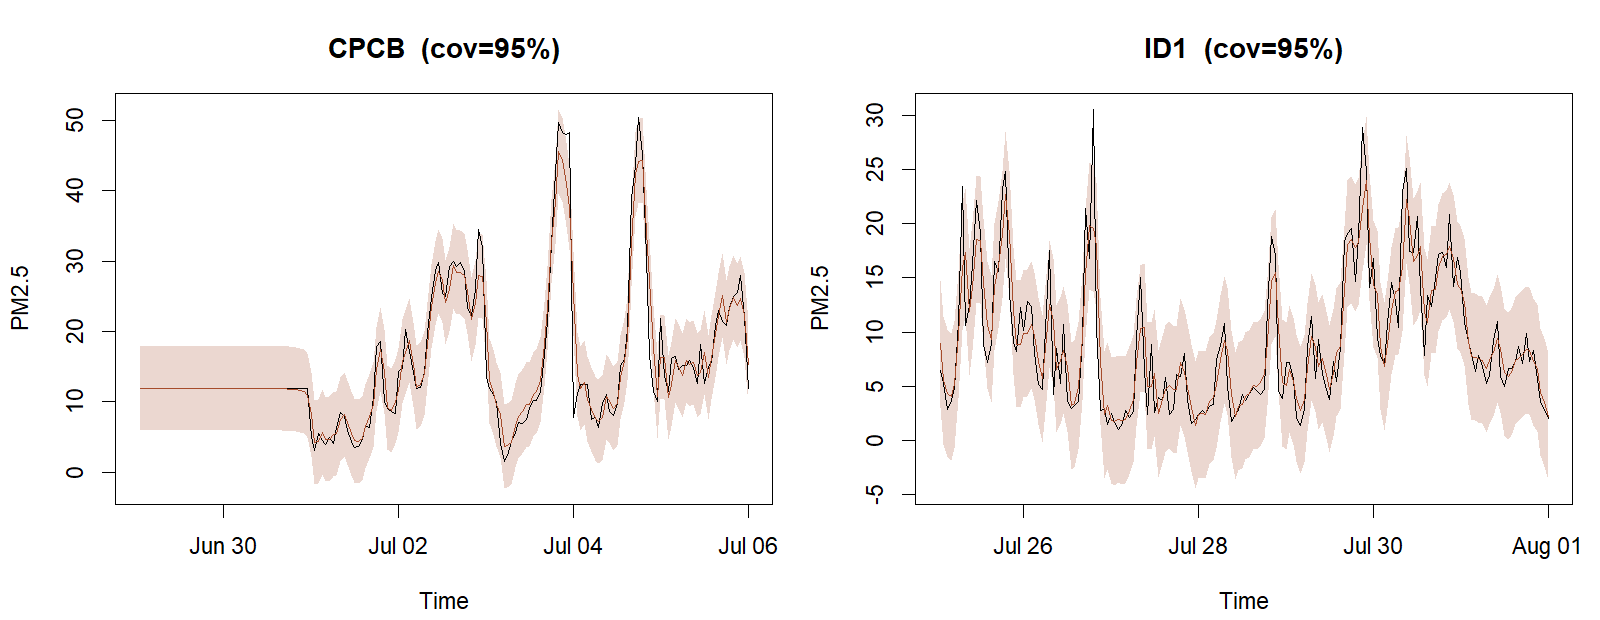
\includegraphics[width=0.98\linewidth,height=0.52\textheight,keepaspectratio]{conformal_cpcb_id1.png}
  \vspace{0.15em}
  {\footnotesize
  \begin{itemize}\setlength\itemsep{0.12em}
    \item \textbf{Black} $=$ actual;\ \textbf{orange} $=$ WaveCatBoost;\
          \textbf{shaded} $=$ 95\% residual PI $[L_t,U_t]$
          (same colours as Rmd §8.2).
    \item Paper residual PI on this window: CPCB / ID1 coverage $\approx 95\%$
          (widths $\approx 12.0$ / $11.7$).
  \end{itemize}
  }
\end{frame}

\begin{frame}{7-day paper residual PI --- summary}
  {\footnotesize
  \centering
  \begin{tabular}{lccc}
    \toprule
    Sensor & Coverage & Mean width & Point MAE \\
    \midrule
    CPCB     & 0.95 & 12.0 & 1.48 \\
    ID1      & 0.95 & 11.7 & 1.96 \\
    Shillong & 0.95 & 19.3 & 3.56 \\
    \bottomrule
  \end{tabular}
  }
  \vspace{0.7em}
  \begin{exampleblock}{Protocol}
    Rolling 1-step WaveCatBoost (letter notebook) + 95\% quantile of
    $|Y-\widehat Y|$ on the plotted 7-day window ($\alpha=0.05$).
  \end{exampleblock}
\end{frame}


\section{Extensions}
% Extensions (from analysis.Rmd §10) — last content section

\subsection{Extensions overview}
\begin{frame}{Extensions --- overview}
  \begin{itemize}\setlength\itemsep{0.4em}
    \item \textbf{Other wavelet filters:} Haar vs D4 vs LA8 (WaveCatBoost).
    \item \textbf{Fourier bands} vs Haar MODWT (WaveLGB).
    \item \textbf{Shillong A0--C3:} input / decomp designs on Lumpyngngad PM$_{2.5}$.
  \end{itemize}
\end{frame}

\subsection{Wavelet filters}
\begin{frame}{Haar vs D4 vs LA8 (WaveCatBoost, 1-day MASE)}
  {\scriptsize
  Same WaveCatBoost head; only the MODWT filter $(p_m,q_m)$ changes
  ($S_{0,t}=Y_t$, indices mod $N$):
  \[
    D_{j,t}=\sum_{m=0}^{M-1}p_m\,S_{j-1,(t-2^{j-1}m)\bmod N},\quad
    S_{j,t}=\sum_{m=0}^{M-1}q_m\,S_{j-1,(t-2^{j-1}m)\bmod N}.
  \]
  }
  {\tiny
  \centering
  \renewcommand{\arraystretch}{1.15}
  \begin{tabular}{@{}l@{\hspace{0.6em}}l@{}}
    \textbf{Haar} ($M{=}2$) &
      $q=(\tfrac12,\tfrac12)$,\ $p=(\tfrac12,-\tfrac12)$ \\
    \textbf{D4} ($M{=}4$) &
      $q\approx(0.483,\,0.837,\,0.224,\,-0.129)$,\
      $p\approx(-0.129,\,-0.224,\,0.837,\,-0.483)$ \\
    \textbf{LA8} ($M{=}8$) &
      $q\approx(-0.076,\,-0.030,\,0.498,\,0.804,\,0.298,\,-0.099,\,-0.013,\,0.032)$ \\
      & $p\approx(0.032,\,0.013,\,-0.099,\,-0.298,\,0.804,\,-0.498,\,-0.030,\,0.076)$ \\
  \end{tabular}
  }
  \vspace{0.25em}
  {\tiny
  \centering
  \resizebox{0.98\linewidth}{!}{%
  \begin{tabular}{llccc llccc}
    \toprule
    Sensor & Pol. & Haar & D4 & LA8 &
    Sensor & Pol. & Haar & D4 & LA8 \\
    \midrule
    CPCB & NO$_2$     & 0.541 & \textbf{0.510} & 0.529 &
    ID1  & NO$_2$     & \textbf{1.252} & 1.346 & 1.330 \\
    CPCB & PM$_{2.5}$ & \textbf{0.727} & 0.909 & 0.955 &
    ID1  & PM$_{2.5}$ & \textbf{0.421} & 0.457 & 0.502 \\
    CPCB & O$_3$      & \textbf{1.014} & 1.212 & 1.119 &
    ID1  & O$_3$      & \textbf{0.935} & 0.940 & 0.964 \\
    CPCB & CO         & \textbf{0.885} & 0.993 & 1.200 &
    ID1  & CO         & \textbf{0.798} & 1.001 & 1.170 \\
    CPCB & SO$_2$     & 6.232 & 6.041 & \textbf{5.972} &
    ID1  & SO$_2$     & \textbf{1.320} & 1.390 & 1.379 \\
    CPCB & PM$_{10}$  & 0.535 & \textbf{0.524} & 0.538 &
    ID1  & PM$_{10}$  & \textbf{0.368} & 0.445 & 0.462 \\
    \bottomrule
  \end{tabular}%
  }
  }
  \vspace{0.2em}
  {\scriptsize
  Haar best on \textbf{9/12} cells; D4 on 2; LA8 on 1 --- Haar stays the default.
  }
\end{frame}

\subsection{Fourier comparison}
\begin{frame}{Fourier vs Haar MODWT (WaveLGB, 1-day)}
  {\footnotesize
  Octave FFT bands matched to Haar layout ($J{=}5$, $p{=}24$).
  Global sinusoids --- no local $D_{1,t}$ (\texttt{extension\_scores}, Rmd §10.1).
  }
  \vspace{0.35em}
  {\scriptsize
  \centering
  \begin{tabular}{llcc}
    \toprule
    Sensor & Pollutant & Haar & Fourier \\
    \midrule
    CPCB & NO$_2$     & \textbf{0.518} & 0.692 \\
    CPCB & PM$_{2.5}$ & \textbf{1.031} & 1.272 \\
    ID1  & NO$_2$     & \textbf{1.259} & 1.438 \\
    ID1  & PM$_{2.5}$ & \textbf{0.360} & 0.473 \\
    \bottomrule
  \end{tabular}
  }
  \vspace{0.45em}
  \begin{itemize}
    \item Haar wins every scored cell.
    \item Fourier smears spikes across frequencies; lags still carry a little of the event.
  \end{itemize}
\end{frame}


\subsection{Shillong study}
\begin{frame}{Shillong: Experiment overview}
  \centering
  {\small Lumpyngngad PM$_{2.5}$: 24, 168, 336 and 744 hours}\par\medskip
  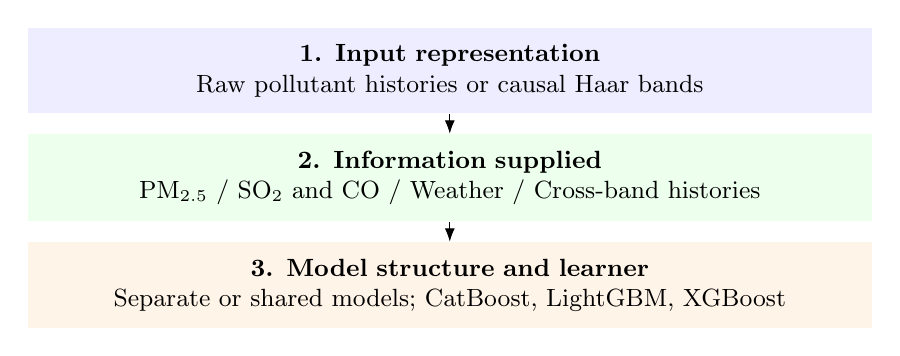
\begin{tikzpicture}[
    box/.style={text width=10.3cm,align=center,inner sep=6pt,font=\small},
    >=Latex
  ]
    \node[box,fill=blue!7] (input) {\textbf{1. Input representation}\\
      Raw pollutant histories or causal Haar bands};
    \node[box,fill=green!7,below=0.25cm of input] (info) {\textbf{2. Information supplied}\\
      PM$_{2.5}$ / SO$_2$ and CO / Weather / Cross-band histories};
    \node[box,fill=orange!9,below=0.25cm of info] (models) {\textbf{3. Model structure and learner}\\
      Separate or shared models; CatBoost, LightGBM, XGBoost};
    \draw[->] (input) -- (info);
    \draw[->] (info) -- (models);
  \end{tikzpicture}
  \par\medskip
  {\small PM$_{2.5}$ forecasts: compare designs across forecast horizons}\par
  {\scriptsize 2023 split: Jan--Jul training / Aug--Sep validation / Oct--Dec test}
\end{frame}

\subsection{Shillong: Raw inputs}
\begin{frame}{Shillong A: Raw-input architectures}
  {\small All designs also use hour-of-day and day-of-week inputs.}\par\medskip
  \scriptsize
  \begin{tabularx}{\linewidth}{@{}p{0.10\linewidth}Xp{0.28\linewidth}@{}}
    \toprule
    Design & Input features & Purpose \\
    \midrule
    A0 & Previous 24 hourly PM$_{2.5}$ values & PM$_{2.5}$ baseline \\[0.7em]
    A1 & A0 + humidity, wind speed, wind direction and rain & Weather information \\[0.7em]
    A2 & Previous 24 hourly values of PM$_{2.5}$, SO$_2$ and CO (72 pollutant inputs) & Other pollutants \\[0.7em]
    A3 & A2 + humidity, wind speed, wind direction and rain & Pollutants + weather \\
    \bottomrule
  \end{tabularx}
  \par\medskip
  A0/A1 use PM$_{2.5}$ history. A2/A3 add SO$_2$ and CO histories.
\end{frame}

\subsection{Shillong: Decomposed inputs}
\begin{frame}{Shillong B: Decomposed PM2.5 inputs}
  {\small Causal Haar decomposition produces six components.}
  \[
    D_1,\ D_2,\ D_3,\ D_4,\ D_5,\ S_5
  \]
  \small
  \begin{tabularx}{\linewidth}{@{}lX@{}}
    \toprule
    Design & Input and modelling setup \\
    \midrule
    B0 & Six PM$_{2.5}$ bands; one model per band \\[0.5em]
    B1 & Same bands; one shared model with a band identifier \\[0.5em]
    B2 & B0 + weather \\[0.5em]
    B3 & B1 + weather \\
    \bottomrule
  \end{tabularx}
  \par\medskip
  B0/B2 fit six separate component models.\par
  B1/B3 use one shared model and a band identifier.
\end{frame}

\subsection{Shillong: Cross-component inputs}
\begin{frame}{Shillong C: Cross-component inputs}
  {\small Can a band benefit from other bands' and pollutants' histories?}\par\medskip
  \scriptsize
  \begin{tabularx}{\linewidth}{@{}p{0.13\linewidth}Xp{0.26\linewidth}@{}}
    \toprule
    Design & Input features & Modelling setup \\
    \midrule
    C1 (sep) & Histories of all six PM$_{2.5}$ bands (144 inputs) & Separate model per band \\[0.5em]
    C1 (sh) & Same C1 information & One shared model \\[0.5em]
    C2 (sep) & Histories of all six bands of PM$_{2.5}$, SO$_2$ and CO (432 inputs) & Separate model per band \\[0.5em]
    C2 (sh) & Same C2 information & One shared model \\[0.5em]
    C3 (sep) & C2 + weather & Separate model per band \\[0.5em]
    C3 (sh) & C2 + weather & One shared model \\
    \bottomrule
  \end{tabularx}
\end{frame}

\subsection{Shillong findings}
\begin{frame}{Shillong: Main findings at Lumpyngngad}
  \small
  \textbf{Multivariate pollutant inputs --- strong benefit}\par
  SO$_2$ and CO histories improve PM$_{2.5}$ forecasts at every horizon.
  \par\medskip
  \textbf{Wavelet decomposition --- no consistent gain}\par
  Raw pollutant histories generally perform better.
  \par\medskip
  \textbf{Weather inputs --- horizon dependent}\par
  Little benefit at 24 h; often worse at longer horizons.
  \par\medskip
  \textbf{Cross-band information --- mixed results}\par
  Helps at 24 and 744 h, but hurts at 168 h.
  \par\medskip
  {\scriptsize Architecture comparisons use LightGBM on the same test targets.}
\end{frame}

\subsection{Boosting-model comparison}
\begin{frame}{Shillong: Boosting-model comparison}
  {\small Same four designs: A0, A3, B0 and C3 (sh). Four forecast horizons.\par
  16 matched test comparisons. Lower mean rank is better.}\par\medskip
  \centering
  \begin{tabular}{lrr}
    \toprule
    Boosting model & Mean rank & Cases won (of 16) \\
    \midrule
    CatBoost & 1.625 & 9 \\
    LightGBM & 2.000 & 4 \\
    XGBoost & 2.375 & 3 \\
    \bottomrule
  \end{tabular}
  \par\medskip
  {\small A3 test MAE by horizon}\par\smallskip
  \scriptsize
  \begin{tabular}{lrrrr}
    \toprule
    Model & 24 h & 168 h & 336 h & 744 h \\
    \midrule
    CatBoost & 8.95 & 10.25 & 12.32 & 11.21 \\
    LightGBM & 9.04 & 10.82 & 12.51 & 12.31 \\
    XGBoost & 10.10 & 11.45 & 14.53 & 13.15 \\
    \bottomrule
  \end{tabular}
  \par\medskip
  CatBoost wins the most matched comparisons among the three boosters.
\end{frame}


\end{document}
